\documentclass[DIV=15]{scrartcl}

\usepackage{fontspec}
\setmainfont{Libertinus Serif}
\setsansfont{Libertinus Sans}
\setmonofont[Scale=MatchLowercase]{Fira Code}

\usepackage{polyglossia}
\setmainlanguage{english}

\usepackage{mathtools}
\usepackage{siunitx}


\usepackage[
  nabla=upright,
  partial=upright,
  bold-style=ISO,
  math-style=ISO,
]{unicode-math}
\setmathfont{Libertinus Math}

\usepackage{graphicx}
\usepackage{wrapfig}

\usepackage{tikz}
\usetikzlibrary{angles}
\usetikzlibrary{quotes}

\usepackage{tikz-3dplot}

\usepackage[labelfont=bf, width=0.9\textwidth]{caption}
\usepackage{subcaption}

\usepackage[urldate=edtf, date=edtf]{biblatex}
\addbibresource{references.bib}

\usepackage[section, below, above]{placeins}

\usepackage[colorlinks, urlcolor=blue!80!black, linkcolor=red!80!black, citecolor=blue!80!black]{hyperref}
\usepackage{bookmark}
\usepackage[shortcuts]{extdash}

\newcommand\azimuth{\ensuremath{\varphi}}
\newcommand\zenith{\ensuremath{\theta}}

\DeclarePairedDelimiter\abs\lvert\rvert
\DeclarePairedDelimiter\norm\lVert\rVert

\usepackage{expl3}
\usepackage{xparse}

\ExplSyntaxOn
\let\vaccent=\v % alten Befehl kopieren
\RenewDocumentCommand \v {} % Befehl überschreiben
{
  \TextOrMath{
    \vaccent % Textmodus
  }{
    \symbf % Mathemodus
  }
}

\NewDocumentCommand \mat {}{\symbf}
\ExplSyntaxOff


\begin{document}
\section{Coordinate System Definition}

\subsection{Horizontal Frame}

In the \emph{Horizontal Frame}, a coordinate in the sky for a given location on earth at a given 
time is represented using the spherical coordinates \emph{Zenith Distance} \zenith{} and \emph{Azimuth} \azimuth{} or cartesian coordinates $\v{r} = (x, y, z)^\top$.
As only the two angles are needed, we normalize the cartesian coordinates, so that $\norm{\v{r}} = 1$.

\begin{figure}[htpb]
  \centering
  \subcaptionbox{%
    3d-coordinates.\label{fig:coords3d}%
  }[0.475\textwidth]{%
    \tdplotsetmaincoords{60}{45}
\begin{tikzpicture}[tdplot_main_coords]
  \draw[thick,->] (0,0,0) -- (3,0,0) node[right]{$x$ (N)};
  \draw[thick,->] (0,0,0) -- (0,3,0) node[right]{$y$ (E)};
  \draw[thick,->] (0,0,0) -- (0,0,3) node[anchor=south]{$z$};

  \pgfmathsetmacro{\ax}{0.5}
  \pgfmathsetmacro{\ay}{2}
  \pgfmathsetmacro{\az}{3}

  \draw[thick,->,red!80!black] (0,0,0) -- (\ax,\ay,\az);
  \draw[dashed,red!80!black] (0,0,0) -- (\ax,\ay,0) -- (\ax,\ay,\az);

  \tdplotgetpolarcoords{\ax}{\ay}{\az}
  \tdplotsetthetaplanecoords{\tdplotresphi}
  \tdplotdrawarc[tdplot_rotated_coords,yellow!60!red]{(0,0,0)}{1}{0}%
    {\tdplotrestheta}{anchor=south,yellow!60!red}{\zenith}

  \tdplotdrawarc[draw=blue!80!black]{(0, 0, 0)}{1}{0}{\tdplotresphi}{anchor=west, blue!80!black}{\azimuth}
\end{tikzpicture}



  }
  \hfill
  \subcaptionbox{%
    Definition of the coordinates in the $x$\-/$y$\-/plane.%
  \label{fig:coords2d}%
  }[0.475\textwidth]{%
    \begin{tikzpicture}

  \draw[thin, lightgray] (0, 0) circle [radius=2cm];
  \foreach \ang in {45, 135, 225, 315} {
    \draw[thin, lightgray, dashed, rounded corners] (0, 0) -- (\ang: 2.8cm)
    node[fill=white] {$\SI{\ang}{\degree}$};
  }

  \coordinate (A) at (0: 2);
  \coordinate (B) at (0, 0);
  \coordinate (C) at (30: 2);

  \draw[->, thick, blue!80!black] (B) -- (C)
  pic [draw=blue!80!black, fill=blue!20, angle radius=1cm, "\azimuth{}"] {angle = A--B--C};

  \draw[->, thick] (-2.2, 0) node[left] {South} -- (2.3, 0) node [right] {$x$  North}; 
  \draw[->, thick] (0, -2.2) node[below] {West} -- (0, 2.3) node [above, align=center, text width=1cm] {East\\$y$}; 

\end{tikzpicture}


  }
  \caption{Coordinate definitions according to astropy.}\label{fig:coords}
\end{figure}

The coordinate system conventions of \texttt{astropy}~\cite{astropy, astropy-coords} are used as shown in \autoref{fig:coords}:
The Azimuth \azimuth{} is $0$ in the North and \ang{90} in the East.
The $x$\-/axis points North, the $y$\-/axis points East and the $z$\-/axis points upwards.

Note that \texttt{astropy} mostly uses \emph{Altitude}, also known as \emph{Elevation}, which is equal to $\ang{90} - \zenith$.

\subsection{Telescope Frame}
\begin{figure}
  \begin{captionbeside}{%
    The Telescope frame: The $z'$-axis is parallel to the pointing vector $\v{p}$ and
    the $x'$-axis is oriented such that the azimuthal angle $\azimuth'$ is
    $0$. 
    The dashed lines show the single coordinate projections for the vector $\v{r}$ in
    the horizontal frame, the dotted lines in the telescope frame.
  }%
    \tdplotsetmaincoords{60}{45}
\begin{tikzpicture}[tdplot_main_coords, scale=3]
  \tikzset{pointing/.style={color=blue!80!black}}
  \tikzset{vector/.style={color=red!80!black}}

  \newcommand\pzd{25}
  \newcommand\paz{20}

  \newcommand\vzd{45}
  \newcommand\vaz{45}

  \pgfmathparse{sin(\vzd)*cos(\vaz)}\let\vx\pgfmathresult
  \pgfmathparse{sin(\vzd)*sin(\vaz)}\let\vy\pgfmathresult
  \pgfmathparse{cos(\vzd)}\let\vz\pgfmathresult


  \tdplotsetcoord{P}{1}{\pzd}{\paz};
  \tdplotsetcoord{R}{1}{\vzd}{\vaz};

  \draw[thick,->, vector] (0,0,0) -- (R) node[right] {$\symbf{r}$};
  \draw[thin, dashed, vector] (Rx) -- (Rxy) -- (Ry);
  \draw[thin, dashed, vector] (Rxy) -- (R);

  \draw[thin, dashed, pointing] (0,0,0) -- (Px) -- (Pxy) -- (Py);
  \draw[thin, dashed, pointing] (Pxy) -- (P);

  \draw[thick,->] (0,0,0) -- (1,0,0) node[right]{$x$ (N)};
  \draw[thick,->] (0,0,0) -- (0,1,0) node[right]{$y$ (E)};
  \draw[thick,->] (0,0,0) -- (0,0,1) node[anchor=south]{$z$};


  \tdplotsetrotatedcoords{\paz}{\pzd}{0}
  \tdplottransformmainrot{\vx}{\vy}{\vz}


  \draw[thick,color=gray,tdplot_rotated_coords,->] (0,0,0) -- (1,0,0) node[right]{$x'$};
  \draw[thick,color=gray,tdplot_rotated_coords,->] (0,0,0) -- (0,1,0) node[left]{$y'$};
  \draw[thick,color=gray,tdplot_rotated_coords,->] (0,0,0) -- (0,0,1.2) node[above right]{$z'$};

  \draw[thin,color=gray,tdplot_rotated_coords, dotted, vector] (\tdplotresx,0,0) -- (\tdplotresx,\tdplotresy,0) -- (0, \tdplotresy, 0);
  \draw[thin,color=gray,tdplot_rotated_coords, dotted, vector] (\tdplotresx,\tdplotresy,0) -- (\tdplotresx,\tdplotresy,\tdplotresz);
  
  \draw[thick,->, pointing] (0,0,0) -- (P) node[right] {$\symbf{p}$};


\end{tikzpicture}




  \end{captionbeside}\label{fig:fact-sensorplane}
\end{figure}
In the \emph{telescope frame}, two angles measured from the optical axis of the telescope are used. One axis is parallel to the Zenith angle and the other axis is perpendicular. 
To transform into this coordinate frame, a coordinate $\v{r}$ given in the horzintal frame as to be rotated according to the pointing direction $\v{p}$ of the telescope,
which is also given as a coordinate in the horizontal frame.


\subsection{Camera Frame}
\begin{figure}
  \begin{captionbeside}{$u$-$v$-coordinate-system for the FACT camera.}
    \begin{tikzpicture}
  \node[anchor=center] at (0, 0.27) {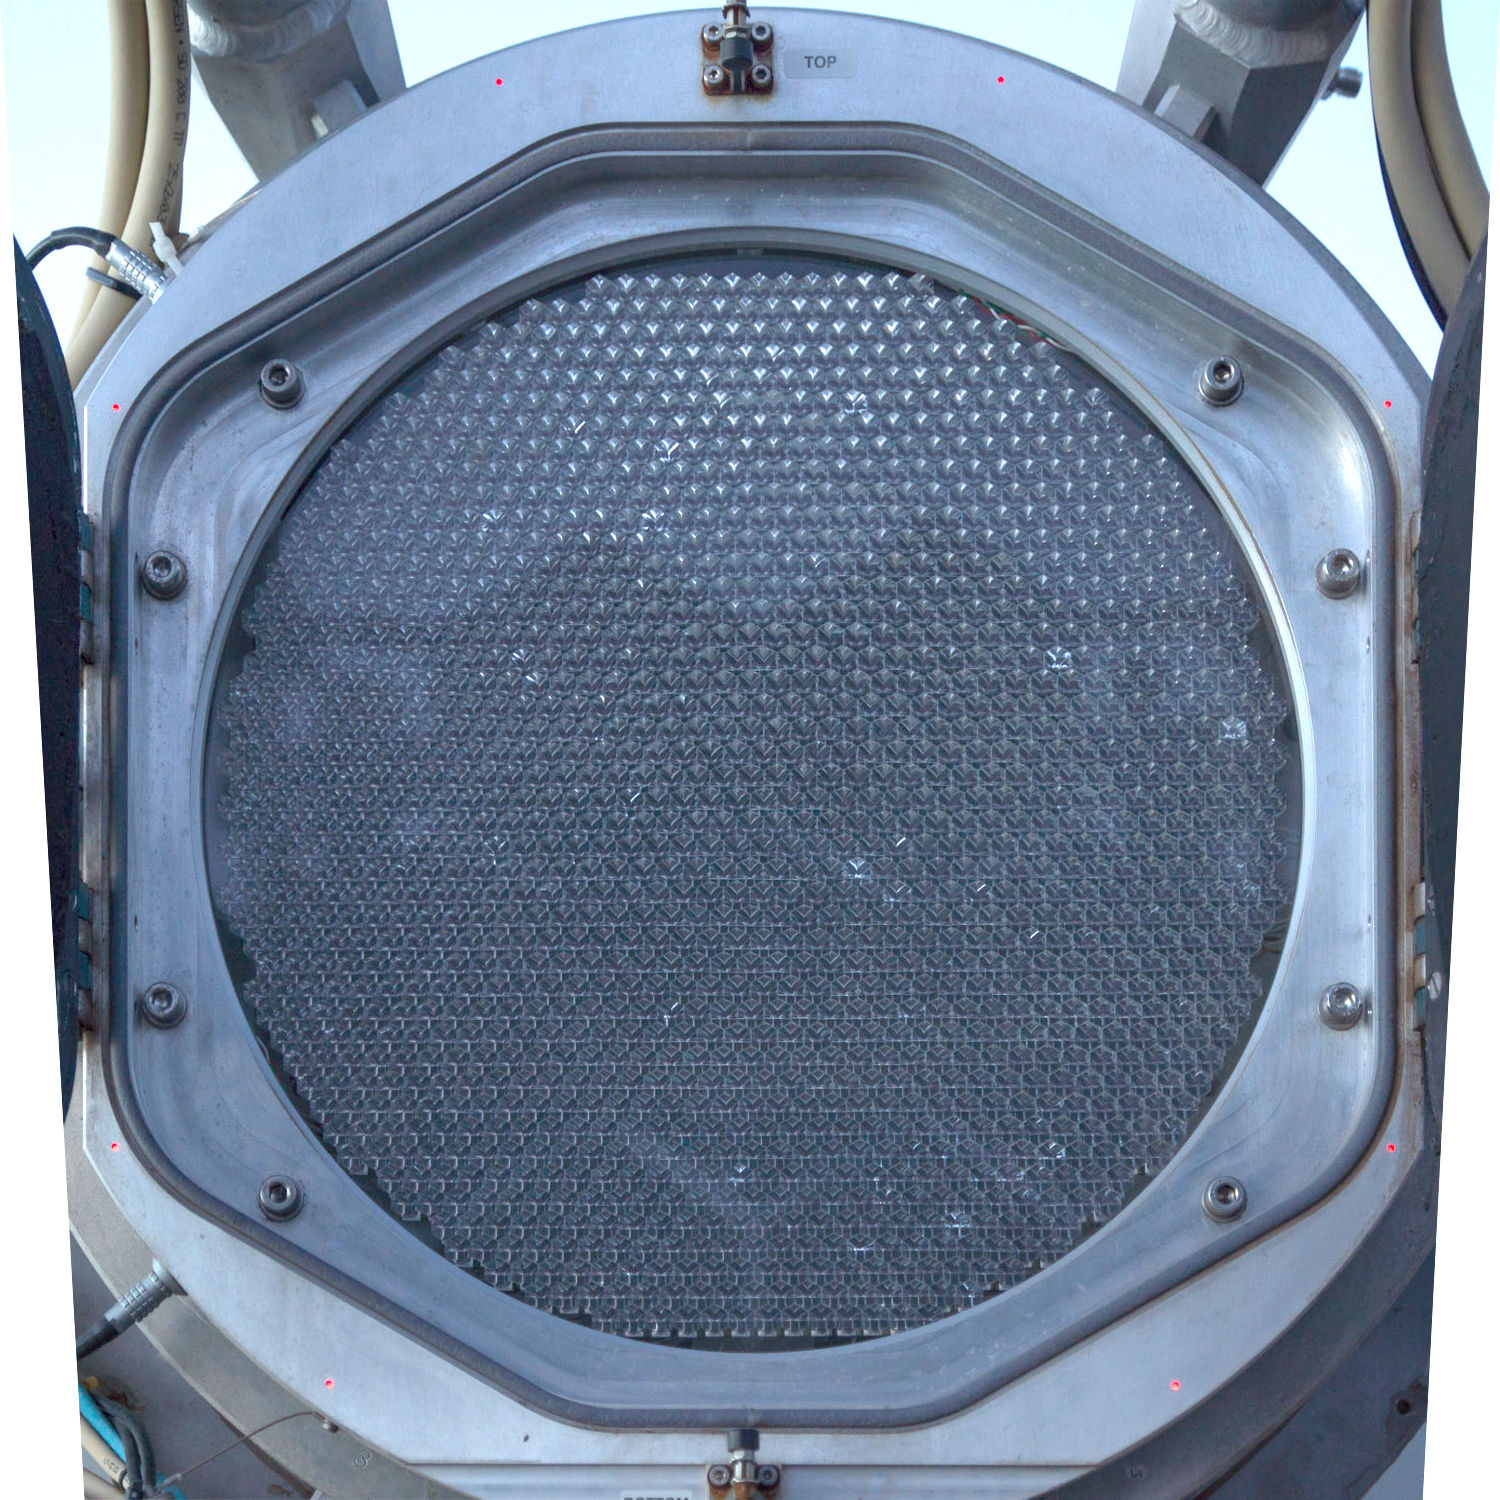
\includegraphics[width=6.6667cm]{graphics/fact_camera.jpg}};
  \draw[very thick, red!80!black, ->] (0, 0) -- (2.5, 0) node[fill=white, right, rounded corners]{$u$};
  \draw[very thick, red!80!black, ->] (0, 0) -- (0, 2.5) node[fill=white, rounded corners, above]{$v$};
\end{tikzpicture}


  \end{captionbeside}
  \label{fig:fact-sensorplane}
\end{figure}

In the \emph{camera} frame, a position is represented by the two cartesian coordinates $u$ and $v$, such that when the sensor plane is watched from the front, $u$ points right und $v$ points upwards.
The case for the FACT camera is shown in \autoref{fig:fact-sensorplane}.
The pixel coordinates for FACT and some other telescopes might be given in coordinate system that is rotated relative to the $u$-$v$-coordinate system.
In the case of FACT, the rotation is \ang{90} counter-clockwise, so mathematically positive.


\section{Transformations}

\subsection{Horizontal Frame ↔ Telescope Frame}
Given the pointing position $\v{p}$ with azimuthal angle 
$\azimuth_p$ and zenith angle $\zenith_p$ in the horizontal frame,
the coordinate angles $\azimuth'$ and $\zenith'$ in the telescope frame for a vector $\v{r}$ with coordinates $\azimuth$, $\zenith$ are calculated by 
using the cartesian representation
and rotating first by $-\azimuth$ around the $z$-axis and then by $-\zenith$ around the $y$-axis and then converting back to spherical coordinates:
\begin{align}
  \v{r}' &= \mat{R}_y(-\zenith) \cdot \mat{R}_z(-\azimuth) \cdot \v{r}
  \intertext{with $\mat{R}_z$ and $\mat{R}_z$ being the \emph{right-handed} rotation matrices\footnote{\texttt{astropy.coordinates.matrix\_utilities.rotation\_matrix} uses the left handed rotation convention.}:}
  \mat{R}_y(\alpha) & =
    \begin{pmatrix} 
      \cos\alpha & 0 & \sin\alpha\\ 
      0 & 1 & 0 \\
      -\sin\alpha & 0 & \cos\alpha
    \end{pmatrix} \\
  \mat{R}_z(\alpha) &=
    \begin{pmatrix} 
      \cos\alpha & -\sin\alpha & 0\\ 
      \sin\alpha & \cos\alpha & 0\\ 
      0 & 0 & 1
    \end{pmatrix}
  \intertext{transforming back to spherical coordinates:}
  \azimuth' &= \operatorname{arctan2}(y, x) \\
  \zenith' &= \arccos(z)
\end{align}




\subsection{Telescope Frame ↔ Camera Frame}

For the conversion from telescope frame to camera frame, the imaging properties of the telescope have to be taken into account.
This boils down to a projection onto the $x'$-$y'$-plane of the telescope frame and then the proper rotation and mirroring for the imaging of the telescope.
Here, only the case of a thin lens approximation for a telescope with given focal length $f$ is discussed.

For a given angle $\alpha$ to the optical axis, the distance to the optical axis $d$ in the image plane for a given focal length $f$ is
\begin{equation}
  d = f \cdot \tan(\alpha),
\end{equation}
or using the small angle approximation, which should be appropriate
for any cherenkov telescope:
\begin{equation}
  d = f \cdot \alpha
\end{equation}
So we get the polar coordinate $r = \sqrt{u^2 + v^2}$ in the camera frame
as 
\begin{equation}
  r = f \cdot \tan{\zenith'} \approx f \cdot \zenith'
\end{equation}
As $v$ should be parallel to the zenith axis we get

\begin{equation}
  u = r \cdot \sin(\azimuth') \\
  v = r \cdot \cos()
\end{equation}


\printbibliography

\end{document}
